% !TEX encoding = UTF-8
% !TEX TS-program = pdflatex
% !TEX root = ../tesi.tex
% !TEX spellcheck = it-IT

%**************************************************************
\chapter{Progettazione}
\label{cap:progettazione-codifica}
%**************************************************************

\intro{In questo capitolo verranno descritte le principali scelte progettuali prese per lo sviluppo dell'ultimo prototipo prodotto. Per una descrizione dettagliata dell'architettura del sistema si rimanda alla specifica tecnica in appendice \ref{appendix:specifica_tecnica}.}\\


\section{Strutture dati}
Per comprendere il sistema è necessario innanzitutto studiare le strutture dati principali che lo compongono.\\

\subsection{Punti e Point Cloud}

\subsubsection{SambaPoint}
\begin{figure}[H] 
    \centering 
    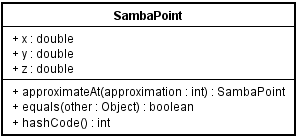
\includegraphics[width=0.7\columnwidth]{diagrammiGenerali/SambaPoint.png} 
    \caption{Diagramma UML della classe SambaPoint}
\end{figure}
La struttura di base, onnipresente nel sistema, è il \texttt{SambaPoint}: è un semplice punto nello spazio descritto dalle sue tre coordinate $x$,$y$ e $z$.//
La classe \emph{SambaPoint} è una estensione di \texttt{Vector3} della nota libreria grafica \emph{Android} \emph{Rajawali3D} al fine di aumentarne la compatibilità con le utilità grafiche offerte da quest'ultima. Come in \emph{Vector3} i campi dati delle coordinate sono pubblici, per aumentare l'efficienza.\\
\texttt{SambaPoint} aumenta le funzionalità della sua superclasse offrendo la possibilità di confronto coordinata a coordinata ed una funzione di approssimazione. 

\subsubsection{Point Cloud di una ricostruzione 3D}
Al fine di memorizzare un oggetto complesso mediante una nuvola di punti si è resa necessaria una nuova struttura dati, più complessa di un semplice insieme di \emph{SambaPoint}.\\
La necessità principale è quella di poter "sommare" due nuvole di punti a patto di conoscere la rotazione e la traslazione relative tra le due. Matematicamente è una semplice trasformazione, ma la sua implementazione su \emph{Point Cloud} molto corposi non è banale; inoltre si è provato sperimentalmente che proprio questa trasformazione è un grosso collo di bottiglia per l'efficienza del sistema: trasformare in maniera poco efficiente una nuvola di migliaia di punti può richiedere anche qualche secondo di elaborazione per ogni rilevazione, rendendo il sistema inutilizzabile.\\
Alla luce di ciò si è scelto di implementare questa struttura dati come \emph{ConcreteStrategy} di uno \emph{Strategy Pattern}, lasciando così la porta aperta a future implementazioni che possano migliorare l'efficienza degli algoritmi.
\begin{figure}[H] 
    \centering 
    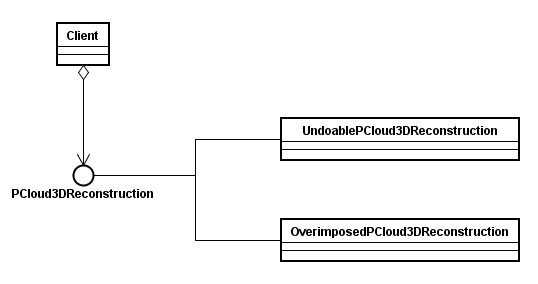
\includegraphics[width=0.9\columnwidth]{diagrammiGenerali/ReconstructionCache.png} 
    \caption{Diagramma UML della classe dell'implementazione dello \emph{Strategy Pattern} per le ricostruzioni 3D}
    \label{fig:reconstruction-strategy}
\end{figure}
La figura \ref{fig:reconstruction-strategy} mostra il diagramma (parziale) dell'architettura usata. Ad esempio si può notare che, oltre alla strategia inizialmente pianificata (ovvero \texttt{OverimposedPCloudReconstruction}), è già stata aggiunta una seconda che permette operazioni di \emph{undo}.\\
Una qualsiasi implementazione di \texttt{PCloud3DReconstruction} rappresenta una nuvola di punti composta da una o più rilevazioni sommate assieme.

\subsection{Stato dell'applicazione}
L'utilizzo medio del prodotto prevede la registrazione di un gran numero di riprese, che devono essere conservate in memoria ed elaborate per fornire un \emph{output} di qualità.

\subsubsection{ReconstructionCache}
\texttt{ReconstructionCache} è una struttura dati piuttosto complessa che tiene memoria di tutte le riprese effettuate e compie ottimizzazioni sui punti immagazzinati.\\
Essa inoltre è uno stato condiviso tra molti \emph{thread} che lavorano concorrentemente; quindi si occupa anche della sincronizzazione e di proteggere opportunamente l'accesso agli stessi in maniera da evitare le potenziali \emph{race condition}.\\
La classe è un \emph{Singleton} in modo da garantire che tutte le componenti che fanno riferimento a quest'ultima facciano riferimento alla stessa istanza.\\
Per l'esterno rappresenta la grande mole di dati che contiene come un unico insieme di punti (che ad esempio può essere rappresentato graficamente come in figura \ref{figure:bidone_conico}). Mentre, al suo interno divide i dati in tre differenti strutture.
\begin{itemize}
	\item Una pila per i \emph{Point Cloud} grezzi ricevuti dai sensori \emph{Tango}, scritti in coordinate relative e che pertanto non possono essere semplicemente sovrapposti gli uni agli altri.
	\item Una struttura dati di ricostruzione 3D (come ad esempio \texttt{UndoablePCloudReconstruction}), che contiene i dati di molte nuvole di punti, correttamente ruotati e sovrapposti tra loro.
	\item Un insieme di punti già ottimizzati: ovvero correttamente approssimati, non ridondanti etc. 
\end{itemize}
Un \emph{Point Cloud} appena catturato viene immediatamente inserito nella pila dei dati grezzi, poi i vari processi di cui è composto il sistema si occuperanno di "spostarlo" da una struttura all'altra fino a farlo giungere nell'insieme dei punti ottimizzati. Nella sezione \ref{section:Servizi} verranno esplicitati i meccanismi con cui ciò avviene.

\subsection{Servizi}\label{section:Servizi}
Come detto nella sezione precedente le operazioni sulle nuvole di punti sono piuttosto dispendiose e quindi impiegano qualche tempo a concludere: non possono, quindi, essere eseguite sullo stesso \emph{tread} che gestisce il resto dell'applicazione. Per questo sono eseguite concorrentemente.
\subsubsection{MergingService e VoxelingService}
\texttt{MergingService} e \texttt{VoxelingService} sono i due servizi che eseguono operazioni sui dati raccolti.
\begin{figure}[!h] 
    \centering 
    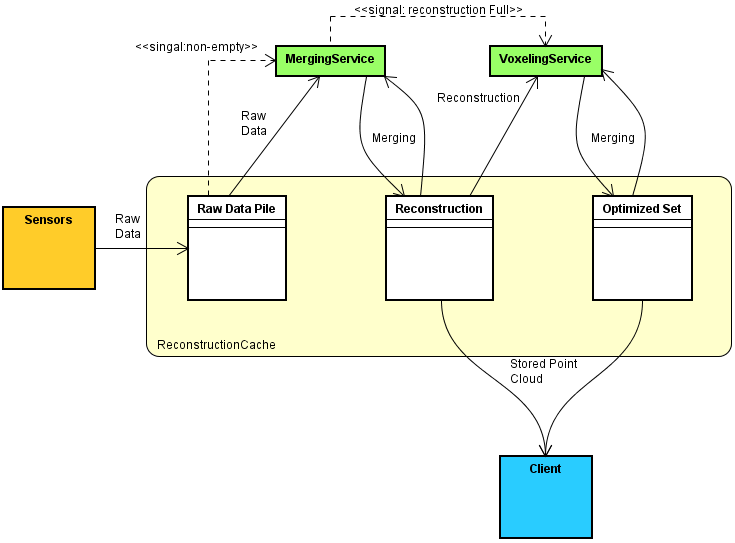
\includegraphics[width=1.0\columnwidth]{diagrammiGenerali/services.png} 
    \caption{Diagramma informale del funzionamento dei servizi di Samba}
    \label{fig:services}
\end{figure}
La figura \ref{fig:services} mostra, in un diagramma informale non UML, il ciclo di vita dei dati all'interno di \texttt{ReconstructionCache}.
\begin{itemize}
	\item Inizialmente i sensori \emph{Tango} inviano i, dati così come li raccolgono, alla \texttt{ReconstructionCache}; vengono posti nella pila.
	\item Quando la pila è non vuota viene lanciato \texttt{MergingService} su un suo \emph{thread}. Quest'ultimo fa il \emph{pop} della pila, ottenendo i dati precedentemente inseriti dal sensore, che sono composti dall'insieme dei punti e da una matrice che descrive la trasformazione che è necessario applicare.
	\item Una volta ottenuti i dati richiede l'accesso alla \emph{Reconstruction} ed effettua la sovrapposizione del \emph{Point Cloud} grezzo con quello (eventualmente vuoto) salvato all'interno della \emph{Reconstruction} stessa.\\Si noti che la \emph{Reconstruction} attualmente viene bloccata dal processo di \emph{merging} anche durante le operazioni di trasformazione del \emph{Point Cloud} grezzo, anche se non ce ne sarebbe bisogno. Ciò è voluto in quanto le operazioni di \emph{merging} saranno soggette a miglioramenti e cambiamenti, quindi potrebbe in futuro rivelarsi necessario fare delle assunzioni sulla \emph{Reconstruction} e non limitarsi alla trasformazione geometrica. A tal proposito si veda la sezione \ref{subs:ICP}.
	\item La quantità di punti all'interno di \texttt{Reconstruction} cresce molto rapidamente. Pertanto il servizio di \emph{merging}, quando il numero di punti supera un tetto prefissato lo segnala al \texttt{VoxelingService}.
	\item \texttt{MergingService} ripete le precedenti operazioni fino a quando non avrà svuotato la pila, al che si addormenterà in attesa di un nuovo segnale.
	\item Il servizio di \emph{voxeling}, svuota \texttt{Reconstruction}, ottimizza i punti (approssimazione e rimozione dei duplicati) e poi aggiunge il risultato ad \texttt{Optimized Set}, ovviamente eliminando altri eventuali duplicati. In questo modo all'interno di \texttt{Optimized Set} ci sarà un \emph{Point Cloud} con punti disposti in una griglia, non sovrapposti e soprattutto in numero molto minore.
	\item Quando i dati vengono inseriti all'interno di \texttt{Reconstruction} vengono già ritenuti "buoni". Infatti quando un \emph{Client} richiede tutti i punti del \emph{Point Cloud} ricostruito si vede ritornare l'unione tra \texttt{Optimized Set} e   \texttt{Reconstruction}.
\end{itemize}

\subsection{Manager}
Sensori \emph{Tango} e \emph{render} grafico hanno un loro ciclo di vita che deve essere gestito all'inteno del ciclo delle \emph{activity} di \emph{Android}.\\
Al fine di separare la logica dell'applicazione dalla sua interfaccia sono stati strutturati dei manager per gestire questi due aspetti: da parte delle \emph{activity} è sufficiente chiamare i metodi di \emph{start} e \emph{stop} coerentemente con il proprio ciclo di vita.\\

%**************************************************************
\newpage
\section{Design Pattern utilizzati}
I \emph{design pattern} sono soluzioni a problemi ricorrenti. Adottare i \emph{design pattern} semplifica
l'attività di progettazione, favorisce il riutilizzo del codice e rende l'architettura
più mantenibile.\\
Nella realizzazione di \emph{Samba} sono stati usati i \emph{design pattern} descritti in questa sezione.

\subsection{MVP}
\subsubsection{Scopo dell'utilizzo}
È stato scelto il \emph{design pattern} \emph{Model View Presenter} per separare la logica dell'applicazione dalla sua rappresentazione e per seguire le \emph{Android Best Practices}.
\subsubsection{Diagramma}
\begin{figure}[H] 
    \centering 
    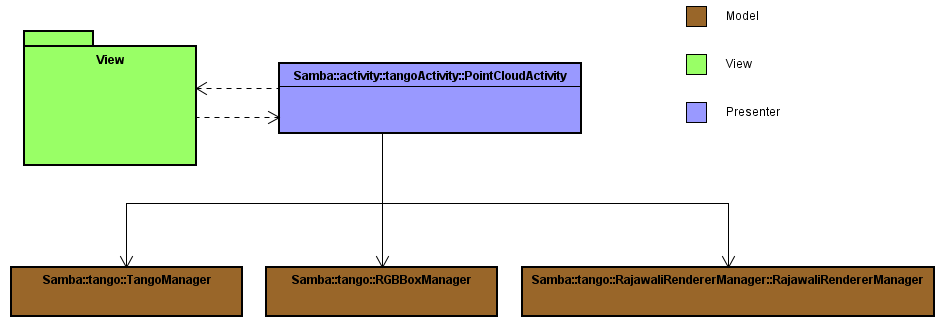
\includegraphics[width=1.0\columnwidth]{st/designPatterns/MVP.png} 
    \caption{Design Pattern MVP, applicazione in Samba}
\end{figure}
Il diagramma spiega la struttura generale di come il pattern MVP è stato utilizzato all'interno di Samba perdendo come esempio una specifica implementazione. Tale implementazione è relativa alla struttura generale del sistema.
\subsubsection{Contesto dell'utilizzo}
Il pattern \emph{MVP} è usato per l'architettura generale del sistema. 

\subsection{Strategy}
\subsubsection{Scopo dell'utilizzo}
Il \emph{Design Pattern} \emph{Strategy} è stato usato per separare la dichiarazione di alcuni algoritmi dalla loro implementazione. Ad esempio negli stadi iniziali non era stato fissato un formato ufficiale per i \emph{file} di \emph{output}; quindi si è lasciata aperta la possibilità di modificarlo in un secondo momento.
\subsubsection{Diagramma}
\begin{figure}[H] 
    \centering 
    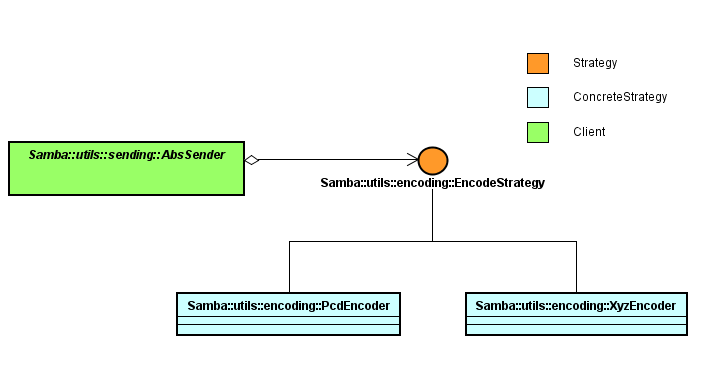
\includegraphics[width=1.0\columnwidth]{st/designPatterns/Strategy.png} 
    \caption{Design Pattern Strategy, applicazione in Samba}
\end{figure}
\subsubsection{Contesto dell'utilizzo}
L'efficienza è un aspetto centrale del sistema, per questo molti algoritmi sono stati implementati mediante \emph{Strategy} per permettere migliorie future.\\
Ad esempio è stato usato uno \emph{Strategy Pattern} per gestire il formato dei \emph{file} in \emph{output}, la rotazione dei \emph{Point Cloud}, le ottimizzazioni sui punti, i servizi per spedire e ricevere informazioni dal \emph{Server} etc.

\subsection{Observer}
\subsubsection{Scopo dell'utilizzo}
Il \emph{Design Pattern} \emph{Observer} è stato usato per permettere l'aggiornamento della \emph{view} da parte dei \emph{manager}.
\subsubsection{Diagramma}\label{dia:ObserverPattern}
\begin{figure}[H] 
    \centering 
    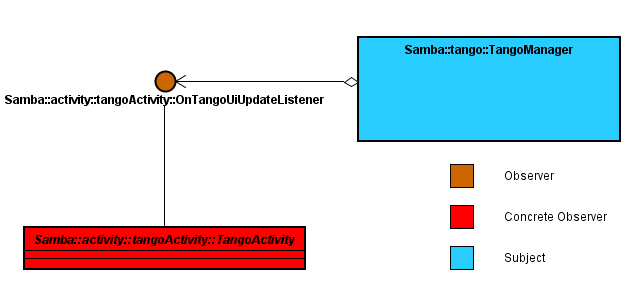
\includegraphics[width=1.0\columnwidth]{st/designPatterns/Observer.png} 
    \caption{Design Pattern Observer, applicazione in Samba}
\end{figure}
\subsubsection{Contesto dell'utilizzo}
È stato usato per permettere l'aggiornamento della view da parte dei \emph{Manager} di:
\begin{itemize}
	\item ciclo di vita \emph{Tango}.
	\item render grafico.
	\item \emph{preview} della fotocamera.
\end{itemize}
Nel diagramma in figura \ref{dia:ObserverPattern} si può osservare il \emph{design pattern} relativo al \emph{manager} del ciclo di vita dei sensori \emph{Tango}.

\subsection{Singleton}
\subsubsection{Scopo dell'utilizzo}
Il \emph{Design Pattern} \emph{Singleton} è stato usato per controllare gli accessi alle classi che mantengono gli stati condivisi tra i vari processi. 
\subsubsection{Diagramma}
\begin{figure}[H] 
    \centering 
    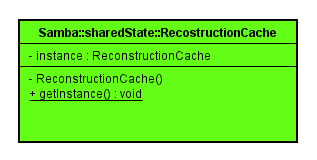
\includegraphics[width=0.5\columnwidth]{st/designPatterns/Singleton.png} 
    \caption{Design Pattern Singleton, applicazione in Samba}
\end{figure}
\subsubsection{Contesto dell'utilizzo}
È stato usato nelle classi che mantengono gli stati condivisi tra i vari processi. Ovvero:
\begin{itemize}
	\item \texttt{Samba.sharedState.ReconstructionCache}
	\item \texttt{Samba.sharedState.ReconstructionManager}	
\end{itemize}




















